\documentclass[a4paper,12pt]{article}

\usepackage{graphicx}
\graphicspath{ {../images/} }


\newcommand{\tab}[1]{\hspace{.1\textwidth}\rlap{#1}}

\begin{document}
	
\begin{titlepage}
	\newcommand{\HRule}{\rule{\linewidth}{0.5mm}} % Defines a new command for the horizontal lines, change thickness here

	\center % Center everything on the page
	 
	
	%----------------------------------------------------------------------------------------
	%	TITLE SECTION
	%----------------------------------------------------------------------------------------

	
	{ \huge \bfseries Software Architecture Requirements and Design Specifications}\\\HRule \\[0.4cm] % Title of your document
	\Large\textbf{Real-time Geospatial Data Processor and Visualizer} \\
	\small \emph{\textbf{Client: Werner Raath}}
	\HRule \\[1.5cm]
	 
	%----------------------------------------------------------------------------------------
	%	MEMBERS, TEAM NAME SECTION
	%----------------------------------------------------------------------------------------
	
\includegraphics[width=\textwidth]{name} \\[1cm]
	\begin{minipage}{0.4\textwidth}
	\begin{flushleft} \large
	
\includegraphics[width=\textwidth]{logo} \\[0.5cm]
	{\large 27 May 2016}\\
	{\large v0.1}
	\end{flushleft}
	\end{minipage}
	~
	\begin{minipage}{0.5\textwidth}
	\begin{flushright} \large
	\emph{Members:}\\% add your name
	Nsovo Baloyi 12163262

	Maluleki Nyuswa 13040686
	
	Keletso Molefe 14222583
	
	Kamogelo Tswene 12163555

	\end{flushright}
	\end{minipage}\\[4cm]
\end{titlepage}


	\newpage
	
	%-------------------------------------------------------------------------------------
	%		TABLE OF CONTENTS
	%-------------------------------------------------------------------------------------
	\tableofcontents
	\newpage
	\section*{Document History}
	\addcontentsline{toc}{section}{\protect\numberline{}Document History}
	
	\begin{table}[h!]
		
		\centering % used for centering table
		\begin{tabular}{c c c c} % centered columns (4 columns)
			\hline\hline %inserts double horizontal lines
			Version & Date & Changed By & Summary \\ [0.5ex] % inserts table
			%heading
			\hline % inserts single horizontal line
			v0.1 & 27 May 2016 & Nsovo Baloyi & First Draft 
			\\ & & Maluleki Nyuswa &  
			\\ & & Keletso Molefe &
			\\ & & Kamogelo Tswene & \\ [1ex] 
			\hline
		\end{tabular}
		\label{table:nonlin} % is used to refer this table in the text
	\end{table}

	\newpage
	
	%-------------------------------------------------------------------------------------
	%		INTRODUCTION
	%-------------------------------------------------------------------------------------
	\section{Introduction}	
	This documentation is the testing documentation for the Geospatial Data Processor and Visualiser project. It outlines the entire testing plan and it documentation process. The documentation firstly establishes the scope, thereafter the testing environment is discussed including all the relevant assumptions and dependencies made during the testing process. The test items, functional features that were tested and the individual test cases are then discussed. Test conducted are then specified according to whether they passed or failed. Test deliverables are then clearly tabulated followed by detailed test results, and finally conclusions and recommendations are noted.

\subsection{Purpose}

This document combines the unit test plan and report into a single coherent artefact. The Geospatial Data Processor and Visualiser system aims to collects geospatial data from third party API's, persist the data on a database and thereafter visualise such in real-time through a web-interface. The system focuses mainly on natural disaster and weather visualisation. 


Software testing forms an integral part of software design, intended to empirically verify whether the software being developed conforms to specifications. Unit testing test a piece of code in isolation against requirements and when done constructively it contributes to code flexibility and and reusability. Black-box testing was used as the tests were developed to contract specification. Test-driven devolopment(TTD) approach was followed during the project as it forms part of the agile development technique.

The benefits of unit testing include:
\begin{enumerate}
	\item[1]Reduced system failure risk.
	
	\item[2]Rapid feedback on developed components.
	
	\item[3]Reduced cost due to
	\begin{itemize}
		\item less time spent on bug fixes
		\item reduced integration problems, and 
		\item lower manual testing costs
	\end{itemize}
	
	\item[4]Improved Maintainability due to unit testing
	
	\item[5]Improved Reusability leading to less code being developed and maintained
\end{enumerate}

\subsection{Scope}

The scope of this document is structured as follows. The features that are considered for testing are listed in section 3. Individual tests that were identified from the requirements are
discussed in detail in section 4. Furthermore, this document outlines the test environment
and the risks involved in the testing approaches that were followed. Assumptions and
dependencies of this test plan will also be mentioned. Section 7.1 and 9 outlines,
discusses and concludes on the results of the tests, respectively.


\subsection{Test Environment}

This section of the document outlines the environment that existed during the unit testing.

\begin{itemize}

	\item Programming Languages:
			AngularJS was primarily used during the development 		stage on the front-end, and NodeJS and ExpressJS on the back-end.
	\item Testing Frameworks:
			Mocha was the primary testing framework used on the back-end. It was chosen for it reach features and ease on testing NodeJS applications. Chai is a TDD assertion library for node and the browser, and was used for it delightfulness for pairing with any testing framework. SinnonJS was used to create mock objects and testing environment.
	\item Coding Environment
			IntelliJ version 9.0 Ultimatum Edition by Jetbrains was the coding IDEA of chose for the project development.
	\item Operating System
			All COEUS team members had the Windows 10 operating system by Microsoft installed on their laptops during the project development stage.
	\item Internet Browsers
			The web-interface was tested to execute accurately on GOOGLE Chrome, Mozilla Firefox and Internet Explorer web browser. 
	
\end{itemize}



\subsection{Assumptions and Dependencies}
\subsubsection{Assumptions}
One of the few assumptions made during the testing was the internet download speed of not less than 5Mb/s. This was important for testing the performance requirements of the system.

\subsubsection{Dependencies}




	
	%-------------------------------------------------------------------------------------
	%		ARCHITECTURE REQUIREMENTS AND APPLICATION DESIGN
	%-------------------------------------------------------------------------------------
	
	\section{Software Architecture Overview}
	Figure 1 shows a high-level overview of the software architecture. In particular, it shows the decomposition of the system into layers with abstract responsibilities, the core architectural components of the system and the concrete frameworks to be used when realizing these architectural components.

\begin{figure}[ht!]
\centering
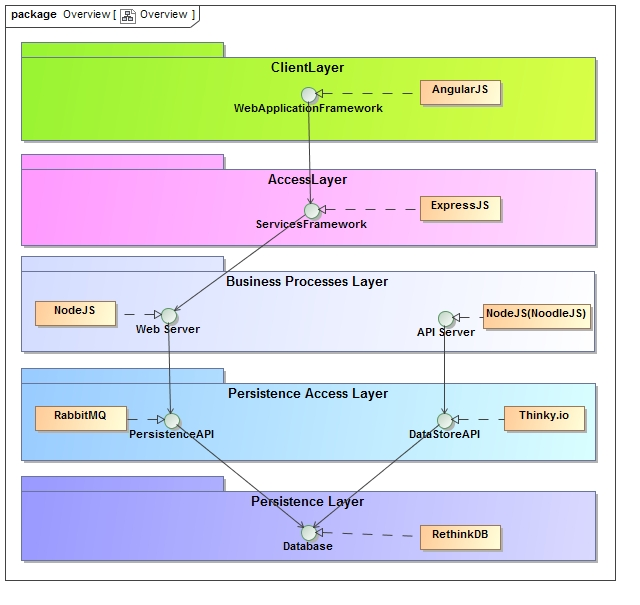
\includegraphics[width=90mm]{../images/Overview.jpg}
\caption{A high-level overview of the software architecture of the Real-time GeoSpatial Data Processor and Visualizer \label{overflow}}
\end{figure}
	
	\section{Architecture Requirements}
	This section specifies the software architecture requirements and the software architecture design
for the system as a whole. The output will be the high level software architecture components, the infrastructure between them and the tactics that will be used to realize the quality requirements for the system. 
	
		\subsection{Architectural Scope}
		In this section discuss architectural responsibilities which need to be addressed by the software
architecture. Typical examples include those of
• providing a persistence infrastructure (e.g. database),
• providing a reporting infrastructure,
• providing an infrastructure for process execution,

		\subsection{Quality Requirements}
		The quality requirements are the requirements around the quality attributes of the systems and
the services it provides. This includes requirements like Flexibility, maintainability, scalability, performance, reliability, security, auditabilty, testability, usability, integrability and deployability requirements.

\subsubsection{Flexibility}  
It is important that the system architecture is designed in such a way that one can easily add different access channels to the system as well a remove old unused or outdated access channels. Furthermore, persistence architectures are evolving at a great rate. The growth of NoSQL databases such as MongoDB and RethinkDB servers as proof of this. In this context it is important that the application functionality is not locked into any specification persistence technology and that one is able to easily modify the persistence provider.

\subsubsection{Maintainability}
Amongst the most important quality requirements for the system is maintainability. It should be easy to maintain the system in the future. To this end
\begin{itemize}
\item future developers should be able to easily understand the system,
\item the technologies chosen for the system an be reasonably expected to be available for a long time,
\item and developers should be able to easily and relatively quickly change aspects of the functionality the system provides.
\end{itemize}

\subsubsection{Scalability}
The purpose of this system is to be used in the business of disaster management, it should allow
for easy scaling in all layers. The system must adhere to the following requirements  
\begin{itemize}
\item The database should support high availability of data,
\item messaging should succeed for every CRUD database operation,
\item and front-end maps should be able to display the geo-spatial information queried by the user.
\end{itemize}

\subsubsection{Performance}
Performance is amongst the most important quality requirements for this system. The following requirements must be considered
\begin{itemize}
\item messages should be small and only supply the most important data, e.g. descriptions and primary keys that could be used by the client to pull data from the API,
\item Front-end maps should react responsively without lag between frames, 
\item the information must be streamed to the user in real-time.
\end{itemize}

\subsubsection{Reliability}
A reliable system allows users to use the system with ease. Users should feel that the system is reliable, to this end
\begin{itemize}
\item client connections to messaging services should never break,
\item server and client exceptions should be handled gracefully.
\end{itemize}

\subsubsection{Security}
Initially the system needs to support only
\begin{itemize}
	\item Users should simply log in and see data relevant to their area of interest. 
	\item HTTPS connections are optional.	
\end{itemize}
In future the system is expected to also enforce confidentiality through encrypted communication and protection against man-in-the-middle attacks through hashing, protect against DOS and DDOS attacks that will stress the servers, and authentication against a chosen user repository (for users who will deploy troops) 

\subsubsection{Auditability}
The system will log all messages processed by the system including all requests and all responses for all user services provided by the system.
For each request and response entries the following will be logged
\begin{itemize}
	\item Request entries:
	\begin{itemize}
		\item an id for the log entry,
		\item the userId of the user requesting the service,
		\item the date/time stamp when the request was made,
		\item the user service requested, and
		\item the request object stringified as JSON with any sensitive information removed.
	\end{itemize}
	
	\item Response entries:
	\begin{itemize}
		\item an id for the log entry,	
		\item the id of the corresponding request entry,
		\item the date/time stamp when the response is provided, and the response object stringified as JSON with any sensitive information removed.
	\end{itemize}
\end{itemize}
The system will provide only services to extract information from the audit log and will not allow the audit log to be modified. Audit logs will be directly accessible to both, humans and systems.

\subsubsection{Testability}
All services offered by the system must be testable through
\begin{enumerate}
\item unit tests,
\item and integration tests
\end{enumerate}

In either case, these tests should verify that
\begin{itemize}
	\item all pre-conditions are met (i.e. that no exception is raised except if one of the pre-conditions for the service is not met), and
	\item that all post-conditions hold true once the service has been provided.
\end{itemize}

In addition to functional testing, the quality requirements like scalability, usability, auditability, performance and so on should also be tested.

\subsubsection{Usability}
Usability is an important quality requirement to consider. The system should be intuitive and efficient to use. Computer literacy is assumed. The time it takes users to find the disaster they're looking for or query a specific disaster should be kept to a minimum. Error handling messages should be self-explanatory and as much as possible of the input validation should be done on the client side.

\subsubsection{Integrability}
The system should be able to easily address future integration requirements by providing access to its services using widely adopted public standards. All use case which are available to human users should also be accessible from external systems.

\subsubsection{Deployability}
Deployability is an important requirement to consider when designing a system. The system should be able to run on any of the 3 most used platforms namely Linux, Windows and Mac OS. The system must:
\begin{itemize}
	\item run on Linux OS,
	\item ultimately the system should be packaged as a Docker image which is deployable on a Docker
container installed on a virtual or physical Linux server.
\end{itemize}


			
		\subsection{Integration and Access Channels Requirements}
		
This section of the document outlines the operability of the system running on the server and demonstrates user access and the integration of different technologies. A Web interface will be the single access channel provided to the user. A detailed discussion follows.\\
\paragraph{Web Interface}
The web interface will be accessed typically through a personal computer using a browser such as Google Chrome, Mozilla Firefox and Internet explorer to name a few.\\
The system will be accessed in the following manner:
\begin{enumerate}
	\item The user will open a web browser of their choice.
	\item Click on the web page where the system will be hosted.
	\item A login page will be displayed.
	\item After user information validation, the user can then have full access to the information they wish to access, based on the privileges assigned to them during user creation.
\end{enumerate}
\subsubsection{Integration Channel Requirements}
Two servers would be used to achieve data persistence, one for interfacing with the website and a second for interfacing with the third-party API for data downloading. The system will also have to interface with a map database (Open Street Map) for downloading maps that will be overlaid with geospatial data. \\
\subsubsection{Protocols}
The only protocol that will be used is HTTP for both the web interface and Android interface. 


The figure below is a simplified explanation of the above text.
\begin{center}
	\includegraphics[scale=0.5]{arch/access_channel.png}
\end{center}
					
		\subsection{Architectural constraints}
		The choice of architecture components and technologies is mostly unconstrained. The development team may choose the architecture and technologies best suited to fulfil the non-functional requirements for the system subject to:
\begin{enumerate}
	\item the system must be deployable in a Docker container, and
	\item the system must use only open source frameworks and tools.
\end{enumerate}

	
	\section{Architectural Patterns}
	The architectural pattern that will be used for the Real-time Geospatial Data Processor and Visualiser system will be the Layering architectural pattern. (See Figure 1)\newline
For the Layering pattern, the layers that will be used are
\begin{enumerate}
	\item Client
		\begin{itemize}
			\item This layer will use the lower layers to have data delivered to it so that it can display the different functionality the user requires in a user friendy manner, which could range from queries to just simply interacting with a map to view what is going on around it.
		\end{itemize}
	\item Access
		\begin{itemize}
			\item This layer, which is a wrapping layer of the business processes layer, makes services available in a technology-neutral way over the Internet. ExpressJS, which is a NodeJS web application server framework, will be used.
		\end{itemize}
	\item Business Processes
		\begin{itemize}
			\item The Business Processes layer will help process requests and will also contain an API server which will be used to extract data from Third Party APIs and/or other reliable data sources.
		\end{itemize}
	\item Persistence Access 
		\begin{itemize}
			\item This layer will be used to access data from the persistence layer, using RabbitMQ to queue messages from the database and it will also be used to write data pulled from public web APIs to the database using Thinky.io.
		\end{itemize}
	\item Persistence
		\begin{itemize}
			\item The persistence layer will manage persistent real-time data which will have been acquired from Third Party APIs. It would in turn supply data, via the Persistence Access Layer, to the Business Logic layer upon request and when there are updates to the requested data.
		\end{itemize}
\end{enumerate}


The Layering pattern is used because:
\begin{enumerate}	
	\item it allows applications to be decomposed into groups of subtasks, each group of subtasks at a certain level of abstraction,
	\item the layers are pluggable and replaceable,
	\item complexity is reduced,
	\item there is loose high-level coupling,
	\item there is ability to mock out lower level layers, and
	\item there is enhanced maintainability
\end{enumerate}
	
	\section{Architectural Tactics}
	Architectural tactics by definition are design decisions that influence the control of a quality attribute response. For the quality attributes identified above, the following are the design decisions that were chosen for some of the quality requirements.

\subsection{Maintainability Tactics}
	Maintainability tactics ensures that the system when modified will preserve its integrity. 
	\begin{enumerate}
		\item Documentation has to always be up to date throughout the entire development process. It should also be self explanatory and be accessible to all who need it.
		\item Another strategy is to localize changes by decomposing all the system elements with clear responsibilities.
	\end{enumerate}
	
\subsection{Scalability and Performance}
	In order to ensure that resource demands are managed efficiently we would do so by: 
		\begin{enumerate}
			\item Reusing resources through using thread pooling and caching. In our system we use thread pooling in the backend system to access and retrieve documents from the database.   
			\item Reducing the load using indexing and optimizing queries which will ensure efiiecient persistence and processing and will also greatly increase the overall speed of retrieving data from the database.
		\end{enumerate}
		
\subsection{Reliability}
	Reliability will be ensured through:
	\begin{enumerate}
		\item Preventing faults using resourc locking and removing single points of failure. This will be done by thorough unit and integration testing throughout development. 
		\item Detecting faults using error/exception communication, in which case if a user wants to use a function/service that they are not authorized to use, an exception message will be communicated to them in a way that the user understands and is able to move forward from and through message integrity by checking that every message or input is valid and not malicious in anyway.
	%\item Recovering from faults by fixing them, rolling back to a state where the system was stable and through maintaing backups.
	\end{enumerate}
	
\subsection{Security}
	\begin{enumerate}
		\item Resisting attacks by limiting access through:
			\begin{itemize}
				\item Minimizing access channels, which at current the system can only be accessed through one access channel taht is the website
				\item Authentication. In order to use any of the functionality in our system, one would need to be registered with the system so that they are able to login.
				\item Authorization. Different users have different access control. A normal user would be able to view and query the system while an admin is able to modify any relevant system data.
			\end{itemize}
		\item Detecting Attacks through monitoring and logging events. 
	\end{enumerate}
	
\subsection{Auditability}
	Auditing will be ensured through
	\begin{enumerate}
		\item Monitoring and logging all messages processed by the system as well as all requests and responses for all the user services.  
		\item Authentication. Every action performed will be linked to the person who has performed it, whether it be a request from a user, a response from the system or admin modifying system data.    
	\end{enumerate}
	
\subsection{Testability}
	\begin{itemize}
		\item Separate interface from implementation. That would allow for substitution of implementations for various testing purposes and would also allow the remainder of the system to be tested in the absence of the component being stubbed.
	\end{itemize}
	
\subsection{Usability}
	\begin{itemize}
		\item Usability will be ensured by making the interface easy to use and having a system that is not cluttered but only has functionality that is necessary.
	\end{itemize}
	
	\section{Reference Architectures and Frameworks}
	Frameworks that are incorporated within our software architecture:
	\begin{enumerate}
		\item AngularJS
			Description: AngularJS is a structural framework used for building dynamic web applications.
			Reasons for using it:
			\begin{itemize}
				\item It is fully extensible, as it lets us extend HTML vocabulary for our application, and it works well with other libraries
				\item It helps with communication between the client and server side, which is helpful fto us as the client and the server communicate regularly to ensure that all the requests made by the client are fulfilled. It tarns async callbacks with promises and deferreds. 
				\item It makes it easy and quick to develop.
				\item It offers two-way data binding between models and views. This data binding allows for an automatic update on both sides whenever there is a data change.
			\end{itemize}
			
		\item ExpressJS
			Description: ExpressJS is a web application framework that provides a set of features for web applications.
			Reasons for using it:
			\begin{itemize}
				\item It is flexible and easy to use
				\item It helps build back-end functions for web applications, which is important for our system as most of the system depends on the functions done in the back-end.
			\end{itemize}
			
		\item Mocha 
			Description: Mocha is a JavaScript test framework which runs on NodeJS
			Reasons for using it:
			\begin{itemize}
				\item It is easier to test async code usind in the back-end. It can run tests in series and also trace exceptions to the right test cases.
				\item It allows for use of any assertion library. In our case we use Mocha with Chai, which is a TDD asertion library.
			\end{itemize}
			
		\item Jasmine
			Description: Jasmine is a behavior-driven development framework.
			Reasons for using it:
			\begin{itemize}
				\item We use it to test our AngularJS application because it has a clean and obvious syntax that makes it easy to write tests for our front-end code.
			\end{itemize}
	\end{enumerate}

	\section{Access and Integration Channels}
		\subsection{Integration Channels}
		The Real-time Geospatial Data Processor and Visualiser system will integrate with:
	\begin{enumerate}
		\item different public web APIs using HTTP requests to pull data.
		\item a database
			\begin{enumerate}
				\item The database will be used to store data which is pulled from the APIs.
				\item The technology that will be used for the database is RethinkDB because it is scalable and will be able to store the massive amount of data that is pulled from the APIs; it also allows for data from the APIs to be stored in real-time, meaning that the data stored would be the most up-to-date at all times (adding new data and updating data that already exists in the database) and it also allows the database to continuously push updated query results to applications in real-time. 
			\end{enumerate}
		\item a messaging service
			\begin{enumerate}
				\item Stores any messages to and from the web client, whether it is an update to the data the web client has already received, or is currently displaying or a new message consisting of different data to the one being currently shown.
				\item In this case the system will integrate with technology, RabbitMQ, which will act as an intermediary for any incoming or outgoing data. 
			\end{enumerate}
	\end{enumerate}

		
		\subsection{Access Channels}
		The Real-time Geospatial Data Processor and Visualiser system will be accessed by different users via the web interface. The web interface will be accessible through web browsers such as Google Chrome, Mozilla Firefox or any other standard web browser.\newline  
The system has two kinds of users, who are:
\begin{enumerate}	
	\item Any person interested in the data
		\begin{itemize}
			\item A user is able to view or track disasters, view weather and they are also able to perform a point or detailed query. A user registered with the system is also able to add, view and edit disaster or weather preferences.
		\end{itemize}
	\item Admin
		\begin{itemize}
			\item An admin user is able to add or modify disaster types as well as access and/or modify relevant system data.
		\end{itemize}
\end{enumerate}


	\section{Technologies}
	Technologies and frameworks that will be used to build the system are as follows:
\begin{itemize}
\item Front-end
\begin{itemize}
	\item AngularJS, provides good RESTFul services and easy integration with other technologies.
	\item RabbitMQ listener as Message bus, to collect real time data from the backend feeder.
	\item Leaflet.js, as our map framework that will use the openStreetMap as its map source.
\end{itemize}
\item Back-end
\begin{itemize}
	\item NodeJS for server-side Web applications.
	\item ExpressJS is a framework for node.js for building web-applications, supports RESTful services.
	\item Bluebird for promises, to complete asynchoneous tasks.
	\item RabbitMQ feeder as Message bus, to collect real time data from the database.
\end{itemize}
\item Database
\begin{itemize}
	\item RethinkDB, supports "changefeeds", which allow you to subscribe to changes on a table. This goes hand in hand with the real-time feature of the system
	\item RabbitMQ, a framework for RethinkDB; is a natural choice for distributing notifications of change events on RethinkDB.
\end{itemize}

\end{itemize}

	
	%-------------------------------------------------------------------------------------
	%		REFERENCES
	%-------------------------------------------------------------------------------------
	
	\section{References}
	\bibliography{references}
	\end{document}
